\documentclass[hyperref, notheorems]{beamer}

% PACKAGES
\usepackage[utf8]{inputenc}
\usepackage{geometry}
\usepackage{appendix}
\usepackage{ytableau}
\usepackage{hyperref}
\usepackage{amsmath}
\usepackage{amssymb}
\usepackage{amsthm}
\usepackage{mathrsfs}
\usepackage{algorithm2e}
\usepackage{tcolorbox}
\usepackage{pgf}
\usepackage{tikz}
\usepackage{tikz-cd}
\usetikzlibrary{arrows,decorations.markings}
\usepackage{pst-platon}
\usepackage{transparent}
\usepackage{graphicx}

% NEW ENVIRONMENTS
\newenvironment{reference}{\begin{tcolorbox}[width=\linewidth,baseline=\tcbtextheight+\baselineskip]}{\end{tcolorbox}}
\newenvironment{creference}{\begin{tcolorbox}[width=\linewidth,baseline=\tcbtextheight+\baselineskip]\centering}{\end{tcolorbox}}

% NEW AND REDEFINED COMMANDS
\newcommand{\legendre}[2]{\genfrac{(}{)}{0.5pt}{0}{#1}{#2}}
\newcommand{\tmod}[1]{\text{ mod }#1}
\newcommand{\xto}[1]{\xrightarrow{#1}}
\newcommand{\xfrom}[1]{\xleftarrow{#1}}
\newcommand{\normal}{\mathrel{\unlhd}}
\newcommand{\mf}[1]{\mathfrak{#1}}
\newcommand{\Mat}{\mathrm{Mat}}
\newcommand{\GL}{\mathrm{GL}}
\newcommand{\SL}{\mathrm{SL}}
\renewcommand{\O}{\mathrm{O}}
\newcommand{\N}{\mathbb{N}}
\newcommand{\Z}{\mathbb{Z}}
\newcommand{\Q}{\mathbb{Q}}
\newcommand{\R}{\mathbb{R}}
\newcommand{\C}{\mathbb{C}}
\newcommand{\F}{\mathbb{F}}
\renewcommand{\H}{\mathbb{H}}
\renewcommand{\P}{\mathbb{P}}
\renewcommand{\a}{\alpha}
\renewcommand{\b}{\beta}
\newcommand{\g}{\gamma}
\renewcommand{\d}{\delta}
\newcommand{\e}{\epsilon}
\newcommand{\z}{\zeta}
\renewcommand{\t}{\theta}
\renewcommand{\i}{\iota}
\renewcommand{\k}{\kappa}
\renewcommand{\l}{\lambda}
\newcommand{\s}{\sigma}
\renewcommand{\o}{\omega}
\newcommand{\vphi}{\varphi}
\newcommand{\emt}{\varnothing}
\newcommand{\x}{\times}
\newcommand{\ox}{\otimes}
\newcommand{\op}{\oplus}
\newcommand{\del}{\partial}
\DeclareMathOperator{\id}{\textrm{id}}
\DeclareMathOperator{\sgn}{\mathrm{sgn}}
\DeclareMathOperator{\im}{\mathrm{im}}
\DeclareMathOperator{\rk}{\mathrm{rk}}
\DeclareMathOperator{\tr}{\mathrm{trace}}
\DeclareMathOperator{\ord}{\mathrm{ord}}
\DeclareMathOperator{\Hom}{\mathrm{Hom}}
\DeclareMathOperator{\End}{\mathrm{End}}
\DeclareMathOperator{\Aut}{\mathrm{Aut}}
\DeclareMathOperator{\Tor}{\mathrm{Tor}}
\DeclareMathOperator{\Ann}{\mathrm{Ann}}
\DeclareMathOperator{\Gal}{\mathrm{Gal}}
\DeclareMathOperator{\Trace}{\mathrm{Trace}}
\DeclareMathOperator{\Norm}{\mathrm{Norm}}
\usepackage{quiver}
\newcommand{\afrak}{\mathfrak{a}}

% BACK OF POCKET TOOLS
% [label=(\roman*)]
% [label=(\alph*)]
% [label=(\arabic{enumi})]

% SPECIAL COMMANDS
\newcommand{\smathcal}[1]{
    \mathchoice
    {{\scriptstyle\mathcal{#1}}}
    {{\scriptstyle\mathcal{#1}}}
    {{\scriptscriptstyle\mathcal{#1}}}
    {\scalebox{.7}{$\scriptscriptstyle\mathcal{#1}$}}
}

% TIKZ PREAMBLE
\newcommand{\disc}{\draw(0,0) [fill=gray] circle (1cm);}
\newcommand{\strip}[1]{
\fill [white,even odd rule,rotate=#1] (1,0) circle[radius=0.42cm] circle[radius=0.28cm];
\fill [lightgray,even odd rule,rotate=#1] (1,0) circle[radius=0.4cm] circle[radius=0.3cm];}
\newcommand{\varstrip}[3]{
\fill [white,even odd rule,rotate=#1] (1,0) circle[radius=0.3*#2+0.12*#3] circle[radius=0.3*#2-0.02*#3];
\fill [lightgray,even odd rule,rotate=#1] (1,0) circle[radius=0.3*#2+0.1*#3] circle[radius=0.3*#2];}
\newcommand{\mstrip}[1]{
\fill [white,rotate=#1] (0.8,0.38) -- (1.25, 0.23) -- (1.43,0.1) -- (1.43,-0.1) -- (1.25,-0.23) -- (0.8,-0.38) -- (0.8,-0.22) -- (1,-0.17) -- (1.3,-0.05) -- (1.3,0.05) -- (0.8,0.22) -- (1,0.17) -- cycle;
\draw [thick,domain=-0.4:0.4,rotate=#1+2.5] plot ({1.4-7*\x*\x}, {\x});
\fill [white,rotate=#1] (1.36,0.01) circle(0.04);
\draw [thick,domain=-0.4:0.4,rotate=#1-2.5] plot ({1.4-7*\x*\x}, {\x});
}
\tikzset{vertex/.style = {shape=circle,draw,minimum size=1.5em}}
\tikzset{edge/.style = {->,> = latex'}}
\tikzset{->-/.style={decoration={
  markings,
  mark=at position 0.55 with {\arrow{stealth}}},postaction={decorate}}}

%BEAMER PREAMBLE
\usefonttheme[onlymath]{serif}
\definecolor{burgundy}{rgb}{0.5, 0.0, 0.13}
\usetheme[sidebarleft]{Caltech}
\setbeamertemplate{footline}[frame number]
\setbeamercovered{transparent}
\theoremstyle{definition}
\newtheorem{definition}{\translate{Definition}}
\newtheorem{theorem}{\translate{Theorem}}
\newtheorem{example}{\translate{Example}}
\newtheorem{conjecture}{\translate{Conjecture}}

% TITLE
\title{Algebraic Connectivity and Spectral Clustering}
\author{Mattie Ji}
\institute{APMA 2812G - Combinatorial Theory}
\date{December 6th, 2022}
\AtBeginSection[]{
  \begin{frame}
    \frametitle{Algebraic Connectivity and Spectral Clustering}
    \tableofcontents[currentsection]
  \end{frame}
}

\begin{document}

\begin{frame}
    \titlepage
\end{frame}

\begin{frame}{Note}
    Throughout this talk, when we say \textbf{``graph"}, we are always considering simple undirected graphs with more than $1$ node.
\end{frame}

\begin{frame}{Notion of Connectivity}
   Throughout this class, we have introduced many notions of connectivity on a graph $G$:
   \begin{itemize}
       \item $\delta(G)$ - the minimum degree of a graph
       \item $v(G)$ - the vertex connectivity of a graph
       \item $e(G)$ - the edge connectivity of a graph
   \end{itemize}
   In this talk, we will introduce a new notion of connectivity.
\end{frame}

\begin{frame}{Algebraic Connecitivity}
\begin{block}{Algebraic Connectivity}
    Let $G$ be an unweighted graph, then the \textbf{algebraic connectivity $a(G)$} of $G$ is the second smallest eigenvalue of the graph Laplacian $L$ of $G$ (including multiplicity).
\end{block}
This is also called the ``Fiedler value" of the graph.

\end{frame}

\begin{frame}{Relation to Connectivity}
Why is $a(G)$ called the \textbf{algebraic connectivity} of $G$?
  \begin{block}{Prop: }
    $a(G) \geq 0$, with the equality achieved if and only if $G$ is disconnected.
\end{block}
The non-negativity of $a(G)$ follows from that fact that $L$ is positive semi-definite.
\begin{block}{Prop: }
    Let $G_1$ and $G_2$ be two graphs with the same vertex sets and $E(G_1) \subset E(G_2)$, then
    \[a(G_1) \leq a(G_2)\]
\end{block}
\end{frame}

\begin{frame}{Relation to other Connectivity}

\begin{block}{Theorem: }
Let $G$ be an unweighted non-complete graph, then we have the following inequality:
\[0 \leq a(G) \leq v(G) \leq e(G) \leq \delta(G)\]
\end{block}

Interestingly enough, when $G = K_n$:
\[v(G) = e(G) = n - 1 < n = a(G)\]
\end{frame}

\begin{frame}{Why $a(G)$?}
Why should we care about algebraic connectivity? What separates it from all the other notions of connectivity we care about?\\
\vspace{\baselineskip}
One reason is that the idea of algebraic connectivity is really simple to generalize for weighted graphs:
\begin{block}{Definition: }
      Let $G$ be a weighted graph, the algebraic connectivity $a(G)$ of $G$ is the second smallest eigenvalue of the graph Laplacian $L$.
\end{block}
\end{frame}

\begin{frame}{Why $a(G)$?}
    
Another reason is that - it turns out algebraic connectivity becomes really relevant in the realms of certain clustering problems.
\begin{block}{Definition: }
      Let $G = (V, E)$ be a weighted graph, and $S \subseteq V$, then the volume on $S$ is
    \[\text{vol}(S) = \sum_{v \in S} deg(v)\]  
\end{block}
\end{frame}

\begin{frame}{The Cut Ratio}
    Let $G$ be a graph with adjacency matrix $A$, let $C_1, C_2$ be a partitioning of its vertices
    \[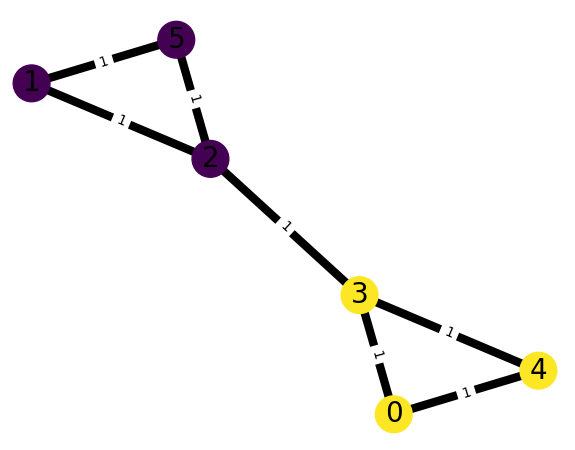
\includegraphics[width=0.5\textwidth]{graphics/g.png}\]
    We define the \textbf{cut-ratio} of $C_1, C_2$ as
    \[[\sum_{v_1 \in C_1, v_2 \in C_2} A_{v_1, v_2}] \cdot (\frac{1}{vol(C_1)} + \frac{1}{vol(C_2)})\]
\end{frame}

\begin{frame}{Spectral Clustering}
\begin{block}{Question:}
    How can we find a partitioning of $V(G)$ such that the cut-ratio is minimized.
\end{block}
    Trying to resolve this is actually NP-Hard, but we can find an approximate solution using the algebraic connectivity of $G$!
\end{frame}

\begin{frame}{The Algorithm}
\begin{algorithm}[H]
\caption{Spectral Clustering}\label{alg:two}
\KwData{The graph $G$ with vertex number $1, 2, ..., n$}
\KwResult{Clusters $C_1, C_2$ partitioning vertices of the graph}
1. Compute the graph Laplacian $L$ of $G$ with ordering of vertices as $1, 2, ..., n$\;
2. Find an eigenvector $v$ of $a(G)$\;
3. Let $v_i$ be the $i$-th component of $v$, then the clusters are $C_1 = \{i: v_i \geq 0\}$ and $C_2 = C_1^c$
\end{algorithm}

\begin{block}{Theorem: }
    If $G$ is a connected graph, then the sub-graph generated by $C_1$ and $C_2$ with respect to $G$ are both connected.
\end{block}
\end{frame}



\begin{frame}{Example}
    Consider the following graph:
    \begin{figure}[ht]
        \begin{minipage}[b]{0.40\linewidth}
            \centering
            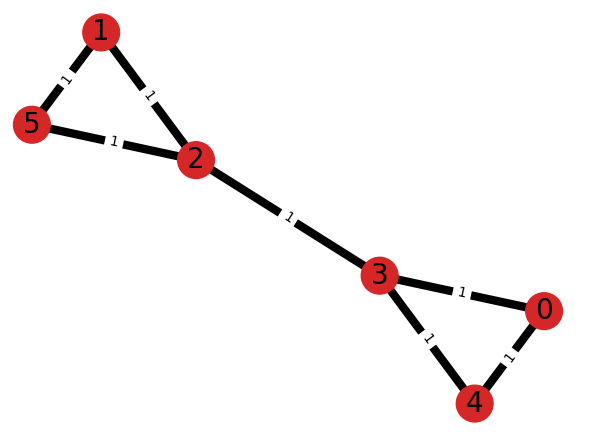
\includegraphics[width=\textwidth]{graphics/raw_g.png}
            \caption{Sample Graph}
            \label{fig:a}
        \end{minipage}
        \hspace{0.5cm}
        \begin{minipage}[b]{0.50\linewidth}
            \centering
            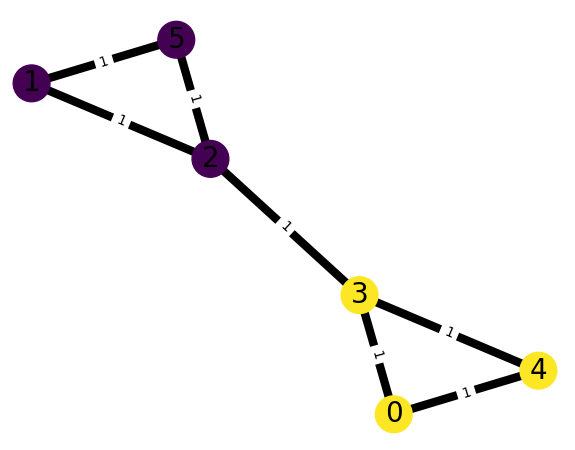
\includegraphics[width=\textwidth]{graphics/g.png}
            \caption{After Running Spectral Clustering}
            \label{fig:b}
        \end{minipage}
    \end{figure}
\end{frame}

\begin{frame}
\frametitle{Spectral Clustering on Data Points}
    In practice, we aren't always going to be handed with a graph. Here's a common scenario
    \begin{block}{Question:}
        Given a list of data-points $p_1, ..., p_n \in \mathbb{R}^d$, how can we partition them in $2$ different clusters?
    \end{block}
    For example:
    \[\frame{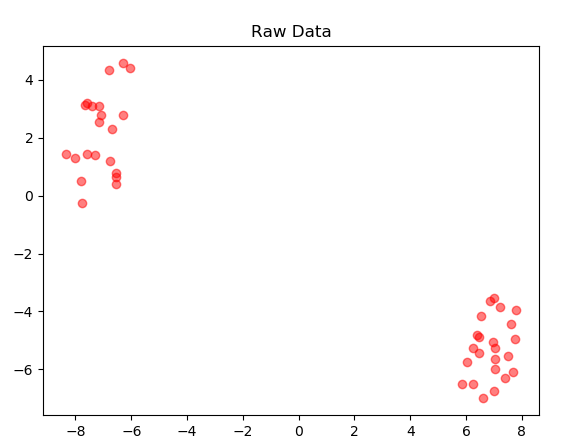
\includegraphics[width=6cm]{graphics/image.png}}\]
\end{frame}

\begin{frame}
\frametitle{Epsilon Neighborhoods}
        The idea here is to create a graph with vertices being the points listed. However, in general there's no one \textbf{correct} way to make these graphs, as it is largely dependent on the domain of the data.\\
        \vspace{\baselineskip}
        There're a few common ways to create the graph:
        \begin{block}{Epsilon Neighborhoods:}
        Let $\epsilon > 0$, for all $i \neq j$, we say that there's an edge of weight $1$
        \[p_i \to p_j \iff d(p_i, p_j) < \epsilon\]
        This will create an undirected graph of uniform weight.
    \end{block}
\end{frame}

\begin{frame}
    \frametitle{Examples of Clustering}
    Here's an example of spectral clustering using the \textbf{Epsilon Neighborhoods} with $\epsilon = 1$
    \[\frame{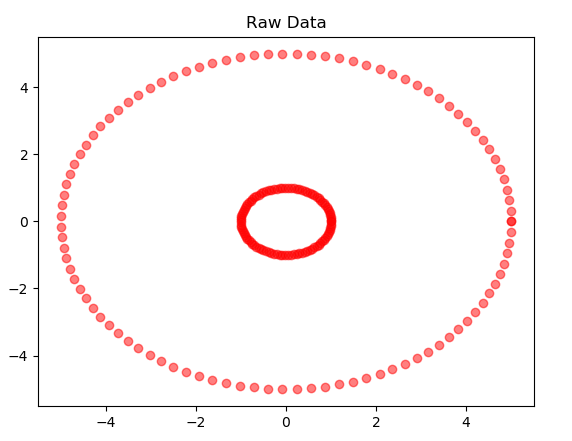
\includegraphics[width=9cm]{graphics/raw_e.png}}\]
\end{frame}

\begin{frame}
    \frametitle{Examples of Clustering}
    Here's an example of spectral clustering using the \textbf{Epsilon Neighborhoods}  with $\epsilon = 1$
    \[\frame{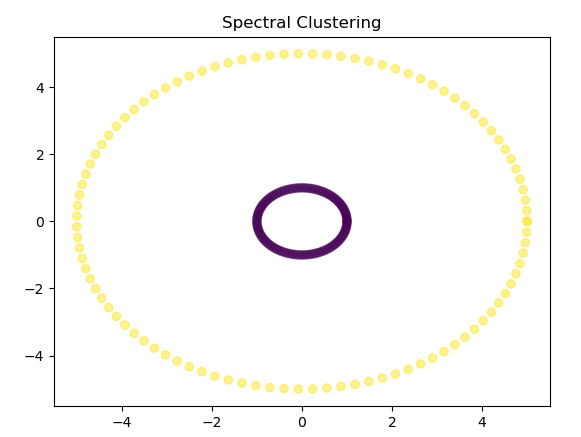
\includegraphics[width=9cm]{graphics/e.png}}\]
\end{frame}

\begin{frame}
\frametitle{Similarity Functions}
    Another idea is to create a fully connected graph and assign weights based on how far they are:
        \begin{block}{Similarity Functions}
        A symmetric function $s: \mathbb{R}^d \times \mathbb{R}^d \to [0, 1]$ is a \textbf{similarity function}. The idea is that $s(x, y) = 1$ means $x$ and $y$ are really close, and $s(x, y) = 0$ means $x$ and $y$ are really far away.
    \end{block}
    The idea is then, for all $i \neq j$, we assign an edge $p_i \to p_j$ of weight $s(p_i, p_j)$.\\
    \vspace{\baselineskip}
    A common choice of similarity function is the \textbf{Gaussian similarity}:
    \[s(x, y) = \text{exp}(\frac{-||x - y||_2^2}{2\sigma^2})\]
\end{frame}

\begin{frame}
    \frametitle{Examples of Clustering}
    Here's an example on our previous example using the with $\sigma = 1$
    \[\frame{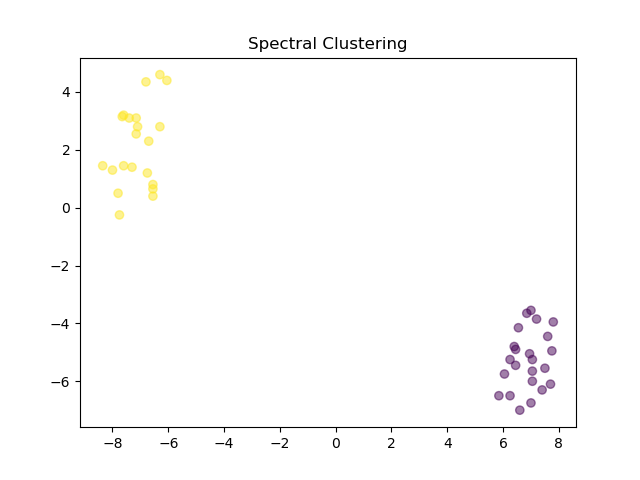
\includegraphics[width=9cm]{graphics/Figure_1.png}}\]
\end{frame}

\begin{frame}{Further Questions}

    \begin{block}{Question:}
What if we want to split into $k$ clusters rather than just $2$?
    \end{block}

    This is totally possible, and the process involves finding the $k$ smallest eigenvalues of $L$ and their respective eigenvectors, but it is beyond the scope of this talk.\\ 
\vspace{\baselineskip}
If you are curious, the details of making $k$ clusters are available on our GitHub:
    \begin{itemize}
        \item[{\includegraphics[scale=.75]{beamericonarticle}}] \url{https://github.com/maroon-scorch/Algebraic-Connectivity}
    \end{itemize}
\end{frame}

\begin{frame}
    \frametitle{Examples of Clustering}
    Here's an example of spectral clustering using the with $\sigma = 1$ and $K = 4$
    \[\frame{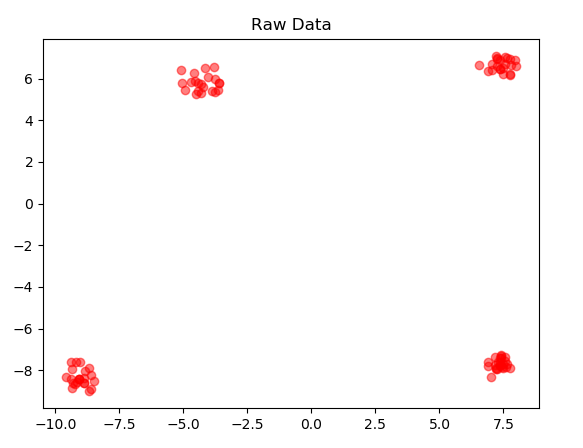
\includegraphics[width=9cm]{graphics/raw_sym.png}}\]
\end{frame}

\begin{frame}
    \frametitle{Examples of Clustering}
    Here's an example of spectral clustering using the with $\sigma = 1$ and $K = 4$
    \[\frame{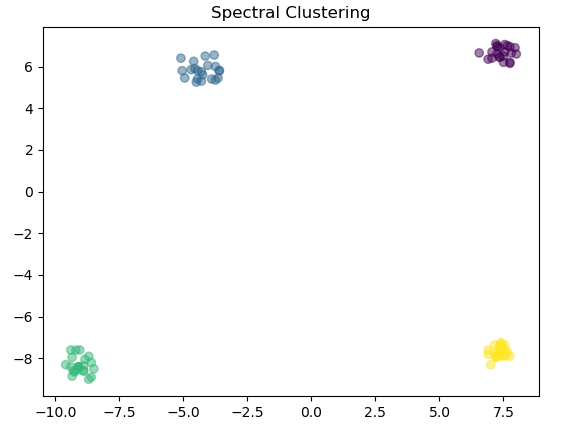
\includegraphics[width=9cm]{graphics/sym.png}}\]
\end{frame}

\begin{frame}{Acknowledgements}
    \begin{itemize}
        \item [1] Fiedler, Miroslav. ”Algebraic connectivity of graphs.” Czechoslovak mathematical journal 23.2 (1973): 298-305.
        \item [2] Fiedler, Miroslav. ”Laplacian of graphs and algebraic connectivity.” Banach Center Publications 25.1 (1989): 57-70.
        \item [3] Strnadová-Neeley, Veronika. ``Spectral Clustering" Seminar on Top Algorithms in Computational Science, 2010. \url{https://sites.cs.ucsb.edu/~veronika/SpectralClustering.pdf}
    \end{itemize}
    All figures and graphs in this presentation were generated by the code repository before.
\end{frame}



\end{document}